% ----------------------------------------------------
% !!!       CHANGE THE COMPILER TO LUALATEX        !!!
% ----------------------------------------------------
\documentclass[a4paper,11pt]{TUmemorandum}
% ----------------------------------------------------
% ---                  CHANGELOG                   ---
% ----------------------------------------------------
% 2023-12-21: 
% added font specifications for Japanese using variable weights
% changed japanese language typesetting support package from 
% xeCJK to luatexja. This requires the use of LuaLaTeX as the
% compiler.
% 
% ----------------------------------------------------
% ---                   PREAMBLE                   ---
% ----------------------------------------------------
% Multilingual support is provided though polygolossa and LuaLaTeX
% Crucially, this allows references to be rendered in both languages 
% In combination with biblatex.
% Please add additinal packages below the biblatex definition to not 
% break the typesetting options.
% CJK support through Google Noto Fonts in LuaLaTeX
\usepackage[style=ieee, language=auto,autolang=langname,]{biblatex}
% Add user packages here
\addbibresource{citations.bib}
% ----------------------------------------------------
% ---               ADRESSING SETUP                ---
% ----------------------------------------------------
% Edit the header section here. You may change the logo
% by uploading a different image and declaring it below.
\memoattention{Bruno Adriano}
\memofrom{Ruben Vescovo}
\memosubject{Monthly meeting 30 November 2023}
\memodate{\today}
\logo{
\includegraphics[width=0.2\textwidth]{tohoku-logo.eps}}
%
\begin{document}
% ----------------------------------------------------
% ---              BEGIN WRITING HERE              ---
% ----------------------------------------------------
\maketitle
% Write your memo text here, and delete \lipsum
% to remove the placeholder text.
\pagestyle{plain}
\section*{Some notes about the template}
%
A few colors are loaded in the class file following the IRIDeS color scheme available from the press-kit logo graphics.\par
\noindent \textcolor{tu}{Lorem ipsum, いづれの御時にか} defined as \verb+tu+
\textcolor{hl}{Lorem ipsum, いづれの御時にか} defined as \verb+hl+ \par
\noindent \textcolor{lg}{Lorem ipsum, いづれの御時にか} defined as \verb+lg+
\textcolor{dg}{Lorem ipsum, いづれの御時にか} defined as \verb+dg+ \par
\noindent \textcolor{or}{Lorem ipsum, いづれの御時にか} defined as \verb+or+
\textcolor{dr}{Lorem ipsum, いづれの御時にか} defined as \verb+dr+ \par
\noindent \textcolor{mg}{Lorem ipsum, いづれの御時にか} defined as \verb+mg+
\textcolor{pbg}{Lorem ipsum, いづれの御時にか} defined as \verb+pbg+ \par
\noindent \textcolor{pv}{Lorem ipsum, いづれの御時にか} defined as \verb+pv+ \par
\noindent to allow some convenience and flexibility. Moreover, the \verb+hyperref+ package is provided with a few custom colors to highlight hyperlinks:
Sample links \url{http://www.tohoku.ac.jp/en/}, \href{https://www.tohoku.ac.jp/japanese/}{masked links}, files \href{run:./LICENSE.md}{LICENSE.md}, English citations~\cite{Koshimura2009a}, Japanese citations~\cite{里美2013}, and figures (Figure~\ref{fig:doggo}).
\begin{figure}[h]
\centering
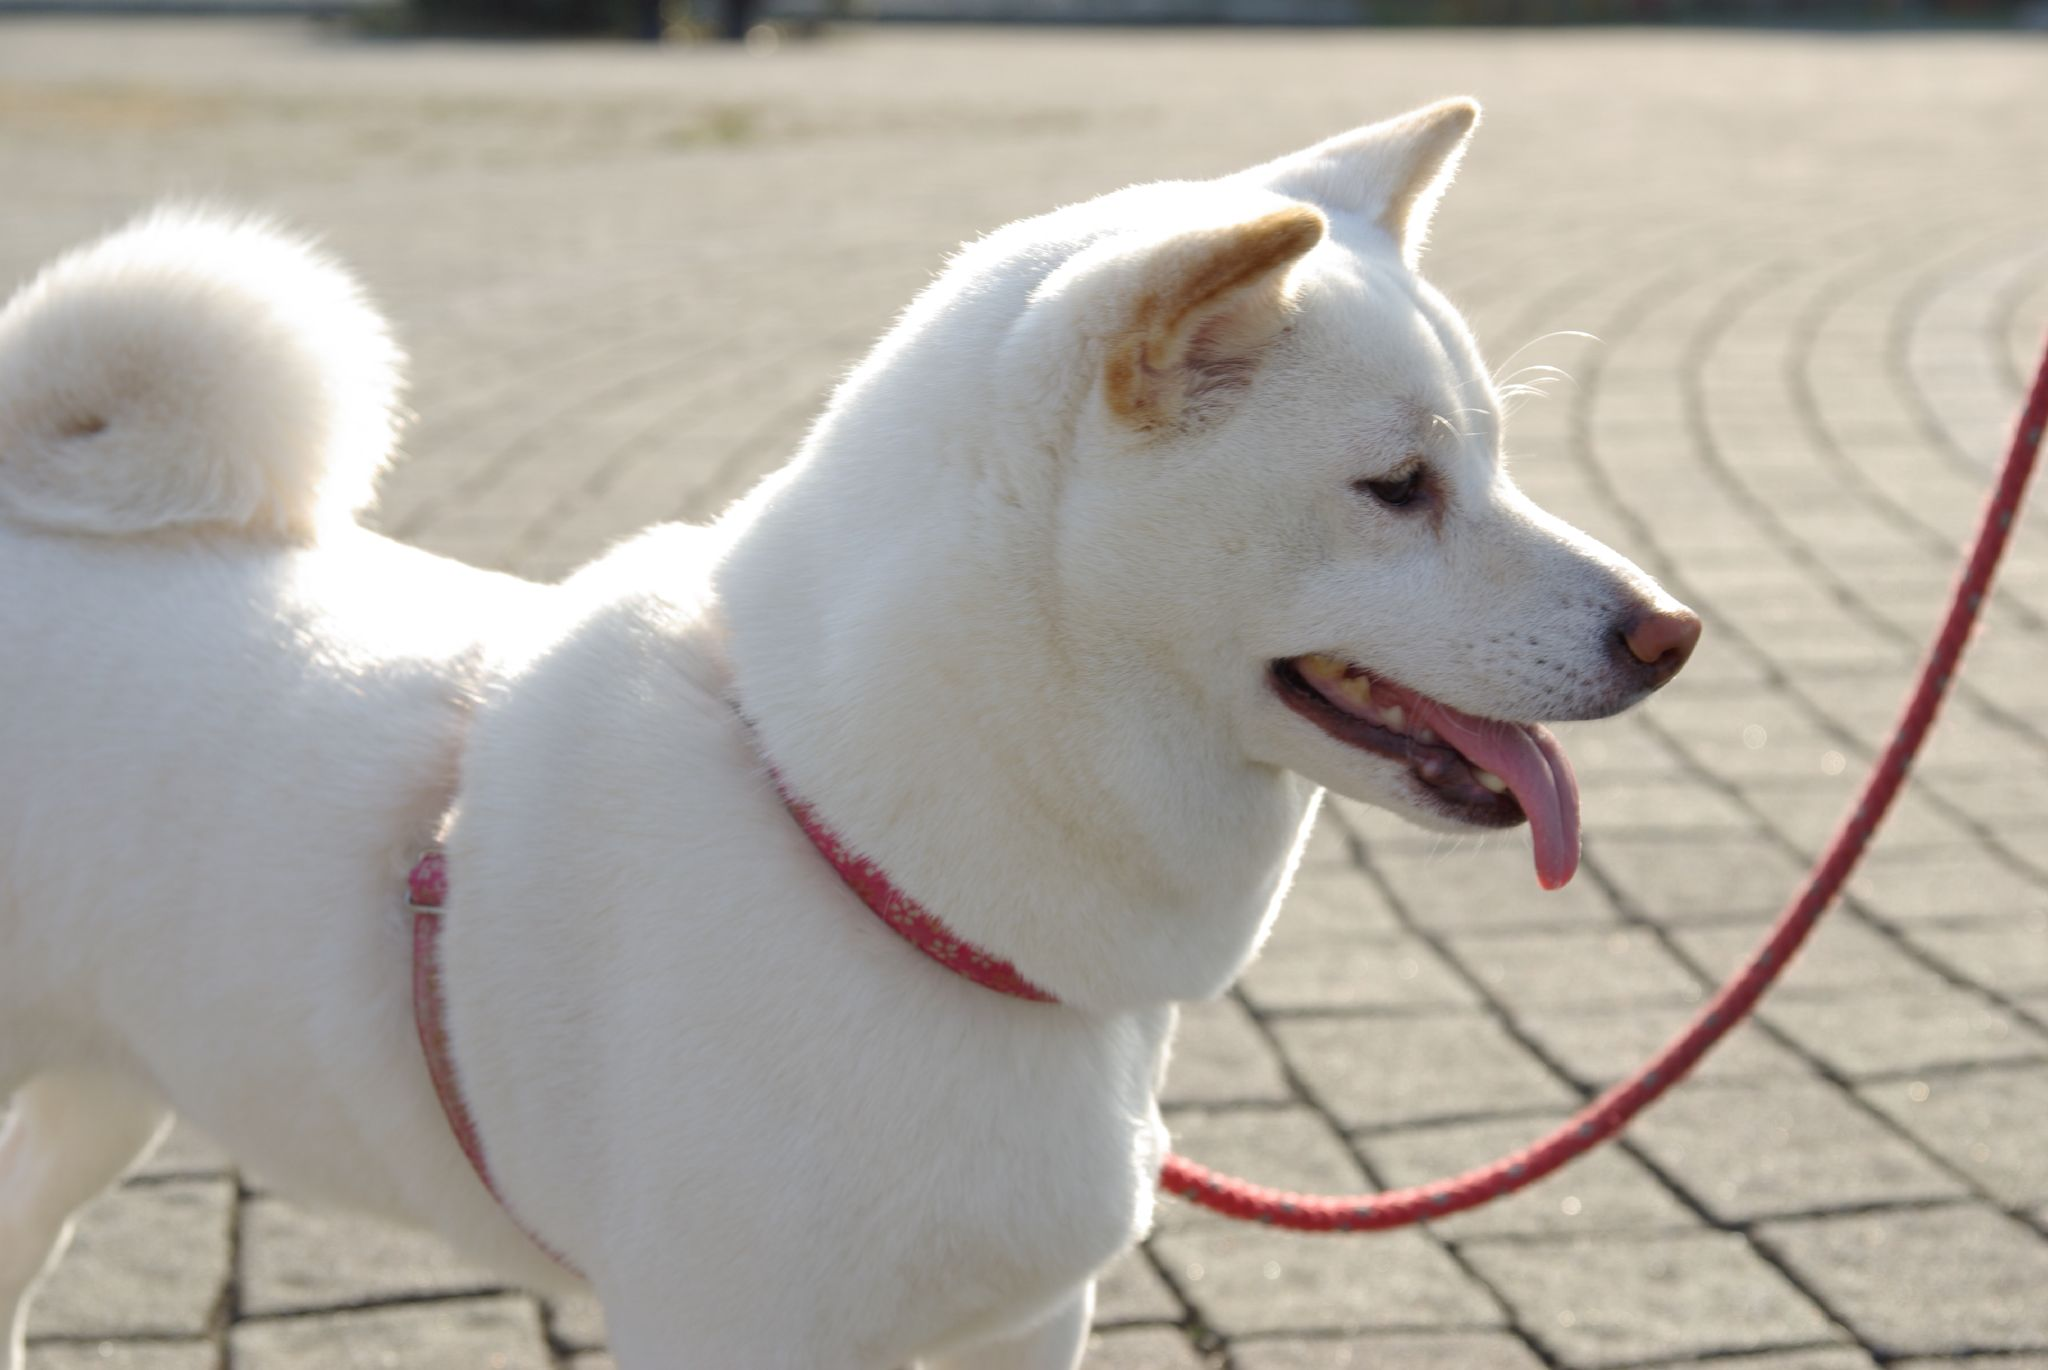
\includegraphics[width=8cm]{shiba.jpg}
\caption{A picture of a good boy.}\label{fig:doggo}
\end{figure}
%
\section*{Lorem ipsum}
%
Lorem ipsum dolor sit amet, consectetur adipiscing elit, sed do eiusmod tempor incididunt ut labore et dolore magna aliqua. Ut enim ad minim veniam, quis nostrud exercitation ullamco laboris nisi ut aliquip ex ea commodo consequat. Duis aute irure dolor in reprehenderit in voluptate velit esse cillum dolore eu fugiat nulla pariatur. Excepteur sint occaecat cupidatat non proident, sunt in culpa qui officia deserunt mollit anim id est laborum.
% \lipsum[1-6] \par
%
\section*{Japanese sample text}
%
いづれの御時にか、女御、更衣あまたさぶらひたまひけるなかに、いとやむごとなき際にはあらぬが、すぐれて時めきたまふありけり。
はじめより我はと思ひ上がりたまへる御方がた、めざましきものにおとしめ嫉みたまふ。同じほど、それより下臈の更衣たちは、ましてやすからず。朝夕の宮仕へにつけても、人の心をのみ動かし、恨みを負ふ積りにやありけむ、いとあつしくなりゆき、もの心細げに里がちなるを、いよいよあかずあはれなるものに思ほして、人の そしりをもえ憚らせたまはず、世のためしにもなりぬべき御もてなしなり。
上達部、上人なども、あいなく目を側めつつ、「いとまばゆき人の御おぼえなり。唐土にも、かかる事の起こりにこそ、世も乱れ、あしかりけれ」と、やうやう天の下にもあぢきなう、人のもてなやみぐさになりて、楊貴妃の例も引き出でつべくなりゆくに、いとはしたなきこと多かれど、かたじけなき御心ばへのたぐひなきを頼みにてまじらひたまふ。
父の大納言は亡くなりて、母北の方なむいにしへの人のよしあるにて、親うち具し、さしあたりて世のおぼえはなやかなる御方がたにもいたう劣らず、なにごとの儀式をももてなしたまひけれど、とりたててはかばかしき後見しなければ、事ある時は、なほ拠り所なく心細げなり。
先の世にも御契りや深かりけむ、世になく清らなる玉の男御子さへ生まれたまひぬ。いつしかと心もとながらせたまひて、急ぎ参らせて御覧ずるに、めづらかなる稚児の御容貌なり。
% ----------------------------------------------------
% ---                BODY ENDS HERE                ---
% ----------------------------------------------------
\printbibliography%
\end{document}